\documentclass[12pt]{article}
\usepackage[top=0.9in, bottom=0.9in, left=0.9in, right=1.1in]{geometry}

\usepackage{graphicx,color,enumitem}
\usepackage{amsmath,amsthm,amsbsy}
\usepackage{palatino}

\usepackage{tikz}

%% Setup aproblem environment, 
%% aproblem items
%% subproblems environment
%% subproblem items
\makeatletter
\newcounter{probcount}
\newcounter{subprobcount}
\newlength\probsep
\newlength\pshrinking
\newif\iffirstprob

\newenvironment{aproblems}%
  {\ifhmode\unskip\par\fi\setcounter{probcount}{0}\probsep\parskip
  \sbox\@tempboxa{\textbf{9.}}\pshrinking\wd\@tempboxa\advance\pshrinking\labelsep
  \let\hproblem\aproblem
  \advance\linewidth -\pshrinking
  \advance\@totalleftmargin\pshrinking
  \advance\leftskip\pshrinking}%
  {\ifhmode\unskip \par\fi\advance\leftskip-\pshrinking}%

\newcommand{\aproblem}{%
  \setcounter{subprobcount}{0}%
  \stepcounter{probcount}%
  \def\@currentlabel{\arabic{probcount}}%
  \ifhmode
    \unskip \par
  \fi
%  \addpenalty{-4000}%
  \iffirstprob\else\addvspace\probsep\fi
  \firstprobfalse
  \hskip -\labelwidth\hskip -\labelsep 
  \hbox to\labelwidth{\hss\textbf{\arabic{probcount}.}}\hskip\labelsep
}%

\newcommand{\subprob}{\item\def\@currentlabel{\arabic{probcount}\alph{\thelistlabel}}}
\newcommand{\skipproblem}{\stepcounter{probcount}}


%% The following commands put defined left and right headers on the top, and a page number
%% on the bottom of all pages beyond page 1
\usepackage{fancyhdr}
\pagestyle{fancy}
\fancyfoot[C]{\ifnum \value{page} > 1\relax\thepage\fi}
\fancyhead[L]{\ifx\@doclabel\@empty\else\@doclabel\fi}
\fancyhead[R]{\ifx\@docdate\@empty\else\@docdate\fi}
\headheight 15pt
\def\doclabel#1{\gdef\@doclabel{#1}}
\def\docdate#1{\gdef\@docdate{#1}}
\makeatother

%% General formatting parameters
\parindent 0pt
\parskip 6pt plus 1pt


\doclabel{Math F251: Section 5.3 Worksheet}
\docdate{Monday 26 November 2018}


\begin{document}
\renewcommand{\d}{\displaystyle}

\begin{aproblems}

% >> plot([0 1 2],[0 2 0],'k','linewidth',2.0),  hold on
% >> x=2:.01:4;  plot(x,-sqrt(1-(x-3).^2),'k','linewidth',2.0)
% >> plot([4 5 6],[0 1 0],'k','linewidth',2.0)
% >> grid on
% >> axis([0 6 -2 3])
% >> ylabel('f(t)','fontsize',24.0)
% >> xlabel('t','fontsize',24.0)
% >> set(gca,'fontsize',20.0)
% >> print -dpdf tentcuptent.pdf
\aproblem \begin{minipage}[t]{0.45\textwidth}  (a) \, The graph of $f(t)$ is at right.  Suppose we define the new function
    $$g(x) = \int_0^x f(t)\,dt$$
Assuming the lines are straight and the curved part is circular, what are the exact values of $g(0),g(2),g(4),g(6)$?
\vspace{2.2in}

\noindent (b) \, Sketch the graph of $g(x)$ on the provided axes.

\bigskip
\noindent (c) \, What is the graph of $g'(x)$?

\bigskip
\end{minipage} \hfill
\begin{minipage}[t]{0.45\textwidth}\vspace{0pt} 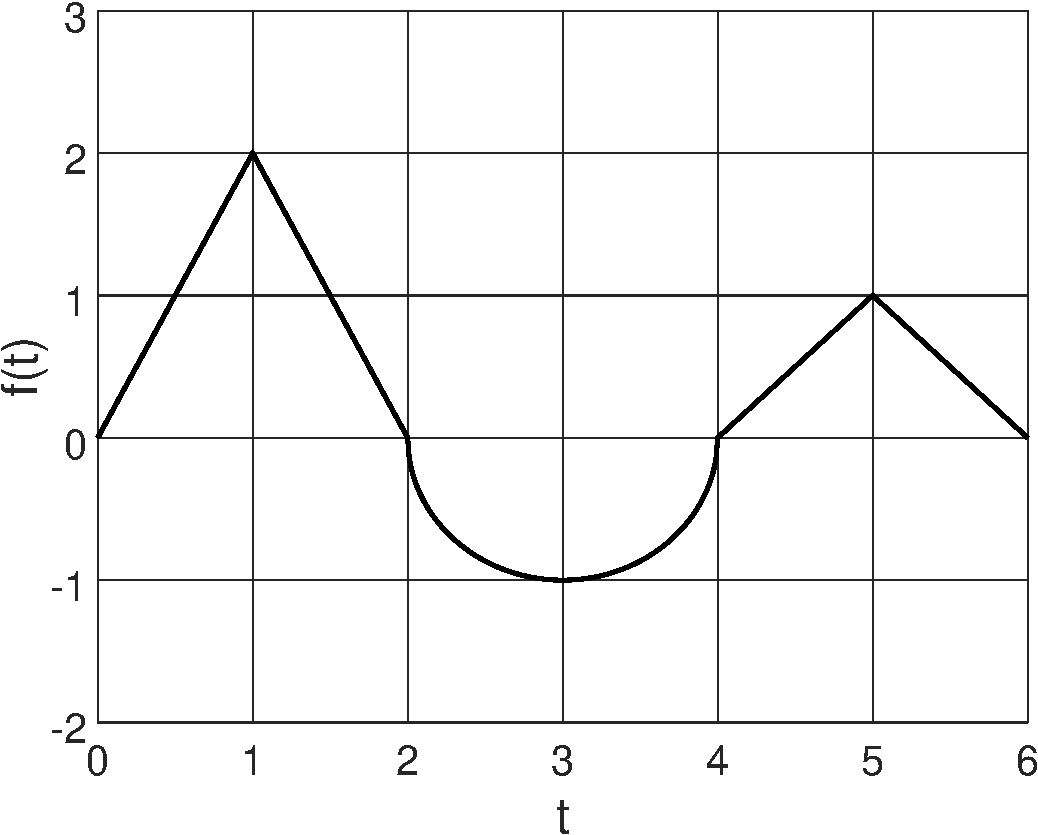
\includegraphics[width=\textwidth]{tentcuptent}

\medskip
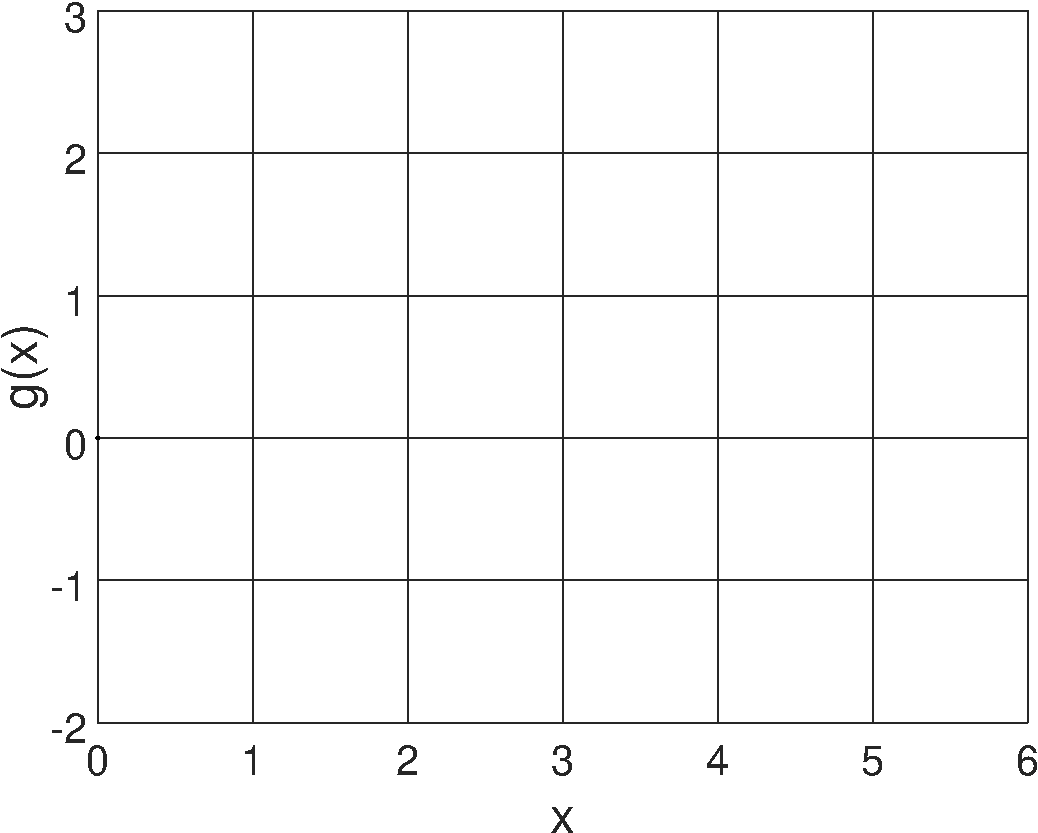
\includegraphics[width=\textwidth]{blankg}
\end{minipage}

\aproblem (a) \quad Use part I of the Fundamental Theorem of Calculus, and the chain rule, to find $dy/dx$ if
    $$y = \int_{\cos x}^\pi \theta^2\,d\theta \hspace{4.0in}$$
\vfill

\noindent (b) \quad Use part II of the Fundamental Theorem of Calculus to find $y=y(x)$.  Then differentiate to find $dy/dx$ \dots and get the same result as in (a).
\vfill

\newpage
\thispagestyle{plain}

% 5.3 % 54
\aproblem Evaluate the integral and interpret as a difference of areas:
    $$\int_{\pi/6}^{3\pi/2} \cos x\,dx = \hspace{4.5in}$$
\vfill

% 5.3 % 39
\aproblem Evaluate the integral:
    $$\int_{1/\sqrt{3}}^{\sqrt{3}} \frac{8}{1+x^2}\,dx = \hspace{4.5in}$$
\vfill

% 5.3 % 33
\aproblem Evaluate the integral:
    $$\int_0^1 (1+r)^3\,dr = \hspace{4.5in}$$
\vfill

% 5.3 % 43
\aproblem Suppose we define a function:
    $$f(x) = \begin{cases} \sin x & \text{if } 0 \le x \le \pi/2 \\
                                          \cos x & \text{if } \pi/2 < x \le \pi \end{cases}$$
Evaluate the integral $\int_0^\pi f(x)\,dx$.
\vspace{2.0in}

\end{aproblems}

\end{document}
